\documentclass{article}
\usepackage{enumitem}
\usepackage[cachedir=minted_cache]{minted}
\usepackage{graphicx}
\graphicspath{ {./img/} }
\usepackage[margin=1in]{geometry} %used to set the margins
\setcounter{secnumdepth}{0} %used to get rid of section numbers
\title{Lab 3 Sorting Pt. 1}
\author{Michael Morikawa}
\date{\today}


\begin{document}
    \maketitle
    \section{Lab Questions}
    \begin{enumerate}[label=\textbf{Question \arabic*}]
        \item What are some good reasons for sorting a list of values? \\
        \textbf{You want to sort a list of values if you are going to be searching for
        those values often so that you can take advantage of binary search algorithms.}
        \item What are the three steps in a divide-and-conquer algorithm design pattern?\\
        \textbf{First step is to divide which means split the input data into different 
        subsets to work with a smaller amount of data. Then you recur which is recursively
         solving the problem with the subsets. Then you conquer which combines the solutions to
         the problems from the subsets.}
    \end{enumerate}

    \section{Source Code}
    \subsection{insertionSort.cpp}
    \inputminted{c++}{../src/insertionSort.cpp}

    \subsection{mergeSort.cpp}
    \inputminted{c++}{../src/mergeSort.cpp}
    \section{Output}
    \subsection{Insertion Sort}
    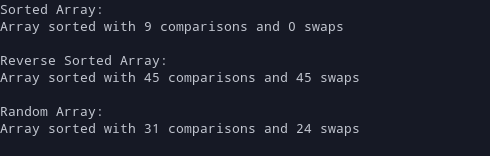
\includegraphics[]{insertionSort.png}
    \subsection{Merge Sort}
    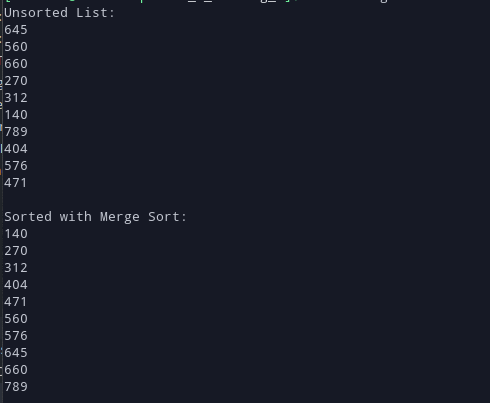
\includegraphics[]{mergeSort.png}
    \subsection{Extra Credit}
    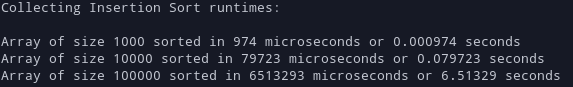
\includegraphics[]{insertionRuntime.png}\\
    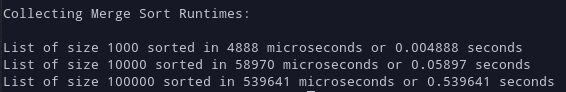
\includegraphics[]{mergeRuntime.png}


\end{document}